\documentclass[12pt,a4paper]{article}
\usepackage[utf8]{inputenc}
\usepackage[russian]{babel}
\usepackage[OT1]{fontenc}
\usepackage{amsmath}
\usepackage{amsfonts}
\usepackage{amssymb}
\usepackage{graphicx}
\usepackage{listings}
\usepackage{xcolor}
\lstset { %
    language=C++,
    backgroundcolor=\color{white!5}, % set backgroundcolor
    basicstyle=\footnotesize,% basic font setting
}
\author{GSench}
\title{Применение различных схем для численного решения уравнения переноса}


\begin{document}

\begin{titlepage}

\begin{center}
\textsc{Федеральное государственное бюджетное образовательное учреждение высшего образования\\
<<Московский государственный университет имени М.В. Ломоносова>>}\\
\vspace{12pt}
\textsc{Механико-математический факультет}\\
\textsc{Кафедра вычислительной механики}\\

\vspace*{\fill}
\textsc{Выпускная квалификационная работа\\
(Дипломная работа)\\
специалиста}\\
\vspace{12pt}
\textsc{\textbf{Применение различных схем для численного решения уравнения переноса}}\\
\vspace*{\fill}

\end{center}

\begin{flushright}
Студент 621 группы \\
Сенченок Григорий Антонович\\
\vspace{10pt}
Научный руководитель: \\
д.ф.-м.н., профессор Меньшов Игорь Станиславович
\end{flushright}

\mbox{}
\vfill
\begin{center}
Москва\\[5pt]
2022
\end{center}

\end{titlepage}

\tableofcontents

\newpage

\section{Аннотация}
Предметом исследования данной работы является цифровое представление нестационарной геометрии на декартовых сетках.
Для данного представления рассматривается численное решение уравнения переноса с помощью метода объема жидкости (Volume of Fluid, VoF). Ключевым моментом реализации данного метода является аппроксимация скачка, который является разрывом характеристической функции, который наблюдается на границе двух сред.
Цель данного исследования - программная реализация и сравнение различных схем геометрической реконструкции разрыва. Были исследованы методы Годунова (константа), MUSCL (линеная функция), THINC (гиперболический тангенс), а также представлен новый метод Jump Reconstruction (JR, восполнение скачком).

\section{Введение}
В данной работе рассматривается проблема численного расчета движения твердого тела в сплошной среде. Твердое тело задано как совокупность точек, лежащих на его границе. Такое представление называется геометрическим. При расчете движения отслеживается положение этих точек, таким образом, происходит моделирование движения в исследуемой области. Проблема геометрического представления заключается в сложности его совмещения с расчетом воздействия на тело сплошной среды. В данной работе представлен способ цифрового представления движения твердого тела.\\
В промышленных системах расчета (например, CAD) для описания геометрии используется метод конечных элементов (МКЭ). На всей исследуемой области вводится сетка, состоящая из простых элементов: для двумерного случая – это многоугольники, для трехмерного – многогранники. Таким образом, происходит точный расчет для большого числа малых конечных элементов, что требует больших вычислительных мощностей для описания каждого примитива и сложного разбиения на эти конечные элементы.\\
В методе, описанном в данной работе, геометрия тела задается характеристической функцией. Данная функция в рассматриваемой области представляет собой индикатор и принимает значение 0, если в рассматриваемой точке находится твердое тело и 1, если жидкость. Эволюцию данной скалярной величины в пространстве и времени описывает уравнение переноса. Такой подход к представлению твердого тела называется цифровой геометрией: Digital Geometry (DG). Это сильно упрощает введение сетки и облегчает расчеты, сохраняя при этом точность на достаточно высоком уровне.\\
Для численного решения уравнения переноса широко используется метод объема жидкости (volume of fluid, VOF). Ключевым моментом реализации данного метода является аппроксимация скачка, который является разрывом характеристической функции, который наблюдается на границе двух сред. Для данного процесса были разработаны различные схемы геометрической реконструкции, позволяющие при использовании их в расчетах метода объема жидкости получить достаточную точность. В данной работе проводится исследование классических способов аппроксимации скачка с помощью константного восполнения: метод Годунова, с помощью линейного восполнения: метод MUSCL. А также проведено исследование альтернативной схемы восполнения гиперболическим тангенсом: метод THINC. При использовании данной схемы была достигнута высокая точность расчетов. Схема THINC - (tangent of hyperbola for INterface capturing) схема отслеживание поверхности с помощью гиперболического тангенса. Также был представлен новый метод численной реконструкции с помощью функции скачка - метод Jump Reconstruction (JR). Данный метод основан на решении обобщенной задачи Римана со смещенным начальным разрывом.\\
В простейшем случае векторное поле, которое воздействует на твердое тело, индуцировано самим твердым телом. Таким образом, расчеты, проведенные для цифровой геометрии возможно сравнить с точным решением. Проблему представления движения в цифровой геометрии можно разбить на две подзадачи: нахождение векторного поля скоростей твердого тела и нахождение характеристической функции твердого тела и жидкости в рассматриваемой области на каждом временном шаге. Первая задача была решена в рамках предыдущей работе. Также была решена задача точного расчета движения твердого тела при известном векторе скорости цента масс и угловой скорости: DirectMotion (DM).\\
Цель данной работы - численная реализация и сравнение различных схем геометрической реконструкции:
\begin{itemize}
  \item метод Годунова
  \item схема MUSCL
  \item метод THINC
  \item метод JR
\end{itemize}


\section{Исследование литературы}

\section{Постановка задачи}


\subsection{Цифровая геометрия}
\subsection{Точное решение: Direct Motion}
Необходимо реализовать программный алгоритм расчета положения твердого тела при движении.\\
Твердое тело представляет собой совокупность точек, расстояния, между положениями которых не изменяются. Известно начальное положение всех необходимых для расчета точек. Одна из точек твердого тела является центром масс. Скорость данной точки известна в любой момент времени. Программа должна рассчитать положение всех точек твердого тела и построить траекторию движения на заданном временном отрезке.\\
Программный алгоритм должен обладать достаточно высокой точностью, для использования результатов его вычислений при расчете движения твердого тела в сплошной среде. Для подсчета точности вычисленного решения предполагается сравнение результатов численного метода с аналитическим решением.\\
Алгоритм должен работать для расчета положения точек тела, как в двумерном, так и в трехмерном пространстве.

\subsection{Уравнение переноса}
\subsection{Jump Reconstruction}

\section{Ограничения и допущения}
При реализации алгоритмов численных методов рассматриваемая область пространства и отрезок времени разбиваются на отрезки равной длины: вводится равномерная сетка с достаточно малой длиной отрезков. Значения искомых величин вычисляются в узлах данной сетки: в определенной клетке пространства и на определенном шаге по времени. Длина и количество отрезков разбиения выбираются таким образом, чтобы полученное численное решение аппроксимировало аналитическое с высокой точностью.\\
При реализации программного алгоритма расчета положения твердого тела при движении для данной задачи мы ограничиваемся двумерным случаем.\\
Граница твердого тела представляет собой многоугольник, состоящий из характерных точек поверхности. Точки считаются характерными точками поверхности, если линию поверхности между двумя соседними точками можно с высокой точностью аппроксимировать прямой линией.\\
При реализации программный алгоритм расчета движения поверхности жидкости для данной задачи мы ограничиваемся пока одномерным случаем. \\
При реализации метода VOF со схемой THINC характеристическая функция может принимать значения в диапазоне от 0 до 1. Значения характеристической функции в таком случае будут показывать объемную долю жидкого и твердого вещества в точке пространства x в момент времени t.\\

\section{Точное решение}
Была решена вспомогательная задача о расчете точного положения точек твердого тела при заданных условиях на скорости и начальное положение.\\
При известном векторе скорости центра масс, векторе угловой скорости твердого тела и начальном положении всех точек твердого тела были численно рассчитаны положения всех точек твердого тела в моменты времени $t_i$.
Расчет был произведен для двумерного случая, но его результаты можно применить и при расчете движения в трехмерном пространстве.
Без ограничения общности рассмотрим задачу точного движения в двумерном случае.

\subsection{Постановка задачи для точного решения}
В двумерное пространство помещено твердое тело, представляющее собой совокупность точек, расстояния, между положениями которых не изменяются. Задана абсолютная система координат.\\
Начальное положение точек твердого тела: $\overrightarrow{x}_k^0 = \overrightarrow{x}_k(0)$, в том числе центра масс:  $\overrightarrow{x}_0^0 = \overrightarrow{x}_c^0 = \overrightarrow{x}_c(0)$.\\
Вектор скорости центра масс: $\overrightarrow{v}=\overrightarrow{v}(t)$. В случае двумерного пространства: $\overrightarrow{v}=(v_x(t), v_y(t), 0)^T$.\\
Вектор угловой скорости твердого тела: $\overrightarrow{\omega}=\overrightarrow{\omega}(t)$. В случае двумерного пространства: $\overrightarrow{\omega}=(0, 0, \omega_z(t))^T$.\\

\paragraph{Дискретизация.}
Введем сетку:\\
Возьмем отрезок времени $T=[0;t]$ и разобьем его на $stepN$ подотрезков $T_i=[t_{i-1}; t_i]$, $i=1..stepN$ - шаги по времени. Длина каждого шага по времени: $\Delta t= t_i-t_{i-1}$. $t_i$ - узлы данного разбиения.\\
Необходимо численно рассчитать положение всех точек $\overrightarrow{x}_k$ твердого тела в узлах  моменты времени $t_i$, $i=1..stepN$.

\subsection{Теоретическая часть}
За скорость любой точки твердого тела отвечает формула Эйлера:
\begin{equation}
\label{eqn:Euler}
\overrightarrow{v}_k(t)=\overrightarrow{v}_c(t)+[\overrightarrow{\omega}(t)\times\overrightarrow{r}_k(t)]
\end{equation}
Где $\overrightarrow{r}_k(t)$ - радиус вектор от центра масс до k-ой точки твердого тела.
\begin{equation}
\overrightarrow{r}_k(t)=\overrightarrow{x}_k(t)-\overrightarrow{x}_c(t)
\end{equation}
\begin{equation}
\overrightarrow{v}_k(t)=\frac{\text{d}\overrightarrow{x}_k}{\text{d}t}
\end{equation}
Подставляя данные значения в уравнение (\ref{eqn:Euler}), получим обычное дифференциальное уравнение для координаты каждой точки твердого тела:
\begin{equation}
\label{eqn:xk_ode}
\frac{\text{d}\overrightarrow{x}_k}{\text{d}t}=\overrightarrow{v}_c(t)-[(\overrightarrow{x}_k(t)-\overrightarrow{x}_c(t))\times\overrightarrow{\omega}(t)]
\end{equation}
Для центра твердого тела данное уравнение имеет вид:
\begin{equation}
\label{eqn:xc_ode}
\frac{\text{d}\overrightarrow{x}_c}{\text{d}t}=\overrightarrow{v}_c(t)
\end{equation}
Интегрирование данного уравнения от 0 до t с использованием начальных условий $\overrightarrow{x}_c(0) = \overrightarrow{x}_c^0$ дает интегральное уравнение для координаты центра твердого тела:
\begin{equation}
\label{eqn:xc_ie}
\overrightarrow{x}_c(t) = \overrightarrow{x}_c^0+\int_{0}^{t} \overrightarrow{v}_c(\tau)d\tau
\end{equation}
Раскрывая разность под векторным произведением в уравнении (\ref{eqn:xk_ode}), получаем:
\[
\frac{\text{d}\overrightarrow{x}_k}{\text{d}t}=\overrightarrow{v}_c(t)-[\overrightarrow{x}_k(t)\times\overrightarrow{\omega}(t)]+[\overrightarrow{x}_c(t)\times\overrightarrow{\omega}(t)]
\] 
Интегрирование данного уравнения от 0 до t с использованием начальных условий $\overrightarrow{x}_k(0) = \overrightarrow{x}_k^0$ дает интегральное уравнение для координаты произвольной точки твердого тела:
\begin{equation}
\label{eqn:xk_ie}
\overrightarrow{x}_k(t)-\int_{0}^{t} [\overrightarrow{x}_k(\tau)\times-\overrightarrow{\omega}(\tau)] d\tau
= 
\int_{0}^{t}(\overrightarrow{v}_c(\tau)+[\overrightarrow{x}_c(\tau)\times-\overrightarrow{\omega}(\tau)])d\tau+\overrightarrow{x}_k^0
\end{equation}

\subsection{Численное решение}
Полученные интегральные уравнения были решены численно методом квадратур.
\paragraph{Центр твердого тела.}
Для решения интегрального уравнения для центра твердого тела (\ref{eqn:xc_ie}) была использована составная квадратурная формула трапеции. Пример программного кода на языке программирования C++ представлен в приложении (\ref{code:xc}) к данной работе.\\
В силу того, что в уравнении отсутствует векторные произведения, а также другие математические конструкции, способные вызвать смешивание координат, возможно разложение векторов по направлениям осей координат и составление решения векторного интегрального уравнения из отдельных решений интегральных уравнений вдоль каждого из направлений Ox, Oy.\\
Таким образом, были получены значения $\overrightarrow{x}_k^i$ сетки в узлах $t_i$ сетки.\\
Не смотря на использование квадратурной формулы трапеции, которая имеет всего лишь 2 порядок сходимости, численные результаты полученные данным методом имеют высокую точность. В силу того, что в качестве скорости центра твердого тела используется гладкая функция, а также за счет достаточно мелкой сетки численное решение получилось крайне близким к аналитическому решению.\\
Полученные значения координаты центра твердого тела в узлах $t_i$ сетки будут использованы в дальнейшем для нахождения векторного поля скоростей твердого тела на декартовой сетке, введенной на исследуемой области. Для этого будет использована та же формула Эйлера для скоростей твердого тела (\ref{eqn:Euler}).
\paragraph{Точка твердого тела.}
Уравнение (\ref{eqn:xk_ie}) также было численно решено методом квадратур. Подход к его решению аналогичен подходу к решению интегрального уравнения Вольтера второго рода. Рассматривается уравнение:
\begin{equation}
\label{eqn:Volter2}
u(x)-\int_{a}^{k} K(x,s)u(s)ds=f(x)
\end{equation}
В данном уравнении присутствуют следующие выражения:
\begin{list}{}{}
\item $x$,$s$ - переменная - параметр
\item $u(x)$ - искомая функция
\item $K(x,s)$ - ядро интегрального уравнения
\item $f(x)$ - функция правой части
\end{list}
В случае интегрального уравнения (\ref{eqn:xk_ie}) для координаты точки твердого тела, параметр $x$ и $s$ - это время $t$ и $\tau$, а функции в уравнении Вольтера имеют вид:\\
Искомая функция:
\[
u(t)=x_k(t)
\]
Произведение функций $K(x,s)u(s)$ в нашем случае является векторным произведением $[\overrightarrow{x}_k(\tau)\times-\overrightarrow{\omega}(\tau)]$, и не зависит от t.\\
$a=0$, при $t=t_0=a=0$\\
Функция правой части:\\
\begin{equation}
\label{eqn:rf}
f(t)=\int_{0}^{t}(\overrightarrow{v}_c(\tau)+[\overrightarrow{x}_c(\tau)\times-\overrightarrow{\omega}(\tau)])d\tau+\overrightarrow{x}_k^0
\end{equation}
Значения данной функции были вычислены аналогично, методом квадратур с использованием составной формулы трапеции. Пример программного кода на C++ расчета значений функции правой части находится в Приложении (\ref{code:rf}).\\
Таким образом, были получены значения                                 $\overrightarrow{f}^i$ вектор - функции $\overrightarrow{f}$ в узлах $t_i$.\\
\[
\overrightarrow{x}_k^0=\overrightarrow{f}(0)=\overrightarrow{f}_0
\]
Применим принцип численного решения интегрального уравнения Вольтера второго рода для вычисления значений $\overrightarrow{x}_k^i$ вектор – функции $\overrightarrow{x}_k(t)$ в узлах равномерной сетки $T_i=[t_{i-1}; t_i]$, $i=1..stepN$. Шаг сетки $\Delta t= t_i-t_{i-1}$. Количество узлов: $stepN+1$.\\
При $t=t_i$ заменим интеграл в левой части уравнения на квадратурную формулу с коэффициентами $A_j^{stepN+1}$:
\[
\overrightarrow{x}_k^i-\Delta x \sum_{j=0}^iA_j^{stepN+1}[\overrightarrow{x}_k^j\times-\overrightarrow{\omega}_j]=\overrightarrow{f}_i+\overrightarrow{R}_i^{stepN+1}(x)
\]
Где $\overrightarrow{R}_i^{stepN+1}(x)$ - погрешность квадратурой формулы. Отбрасывая данную малую величину, решим систему уравнений относительно $\overrightarrow{x}_k^i$, $i=0..stepN$.
\[
\overrightarrow{x}_k^i-\Delta x \sum_{j=0}^{i-1}A_j^{stepN+1}[\overrightarrow{x}_k^j\times-\overrightarrow{\omega}_j]-\Delta x A_i^{stepN+1}[\overrightarrow{x}_k^i\times-\overrightarrow{\omega}_i]=\overrightarrow{f}_i
\]
\begin{equation}
\label{eqn:xk_slae}
\overrightarrow{x}_k^i-[\overrightarrow{x}_k^i\times-\Delta x A_i^{stepN+1}\overrightarrow{\omega}_i]=\overrightarrow{f}_i+\Delta x \sum_{j=0}^{i-1}A_j^{stepN+1}[\overrightarrow{x}_k^j\times-\overrightarrow{\omega}_j]
\end{equation}
Введем новые обозначения:
\begin{list}{}{}
\item $\overrightarrow{x}_k^i=\overrightarrow{x}$
\item $-\Delta x A_i^{stepN+1}\overrightarrow{\omega}_i=\overrightarrow{b}$
\item $\overrightarrow{f}_i+\Delta x \sum_{j=0}^{i-1}A_j^{stepN+1}[\overrightarrow{x}_k^j\times-\overrightarrow{\omega}_j]=\overrightarrow{c}$
\end{list}
Тогда уравнение (\ref{eqn:xk_slae}) примет вид:
\[
\overrightarrow{x}-[\overrightarrow{x}\times\overrightarrow{b}]=\overrightarrow{c}
\]
\[
\overrightarrow{x}+[\overrightarrow{b}\times\overrightarrow{x}]=\overrightarrow{c}
\]
Заменим операцию векторного произведения на произведение кососимметрической матрицы на вектор.
\[
\overrightarrow{x}+[\overrightarrow{b}]_{\times}\overrightarrow{x}=\overrightarrow{c}
\]
\[
(E+[\overrightarrow{b}]_{\times})\overrightarrow{x}=\overrightarrow{c}
\]
\[
\overrightarrow{x}=(E+[\overrightarrow{b}]_{\times})^{-1}\overrightarrow{c}
\]
Матрица $E+[\overrightarrow{b}]_{\times}$ была рассчитана для двумерного случая, однако можно использовать тот же способ для расчета в трехмерном пространстве.\\
Таким образом, мы выражаем вектор $x_k^i$ для $i=0..stepN$. Вектор $x_k^i$ необходимо рассчитывать последовательно, так как в сумме $\sum_{j=0}^{i-1}A_j^{stepN+1}[\overrightarrow{x}_k^j\times-\overrightarrow{\omega}_j]$ используются значения $x_k^j$ для $j=0..i-1$.\\
В качестве квадратурной формулы была использована комбинация составной формулы Симпсона и правила трех восьмых.\\
В результате была реализована программа для вычисления положений k-ой точки твердого тела в моменты времени $t_i$,$i=0..stepN$.\\
Пример программного кода, реализующий данный алгоритм находится в Приложении (\ref{code:xk}).

\subsection{Пример расчета}
Вектор – функции в данной программе задаются с помощью лямбда - выражений на языке программирования C++, что обеспечивает высокую гибкость в настройке программы под любую конфигурацию задачи. Например, вектор - функция скорости центра масс твердого тела может быть задана следующим образом:
\begin{lstlisting}
function<VectorXd(double)> v = [=](double t)->VectorXd {
        VectorXd v(n);
        v(0) = 1;
        v(1) = 50 - 9.81 * t;
        return v;
    };
\end{lstlisting}
Для демонстрации работы программы было выбрано твердое тело, состоящее из 12 точек, которые в начальный момент времени имели следующие координаты:

Вектор угловой скорости:
\begin{lstlisting}
function<Vector3d(double)> omega = [=](double t)->Vector3d {
    return Vector3d(0, 0, 1);
};
\end{lstlisting}
Количество шагов и длина шага сетки:
\begin{lstlisting}
int stepsN = 100;
double h = 0.1;
\end{lstlisting}
Координаты выбранных точек твердого тела записаны в файле output.txt и имеют следующий вид:
\begin{figure}[h!]
  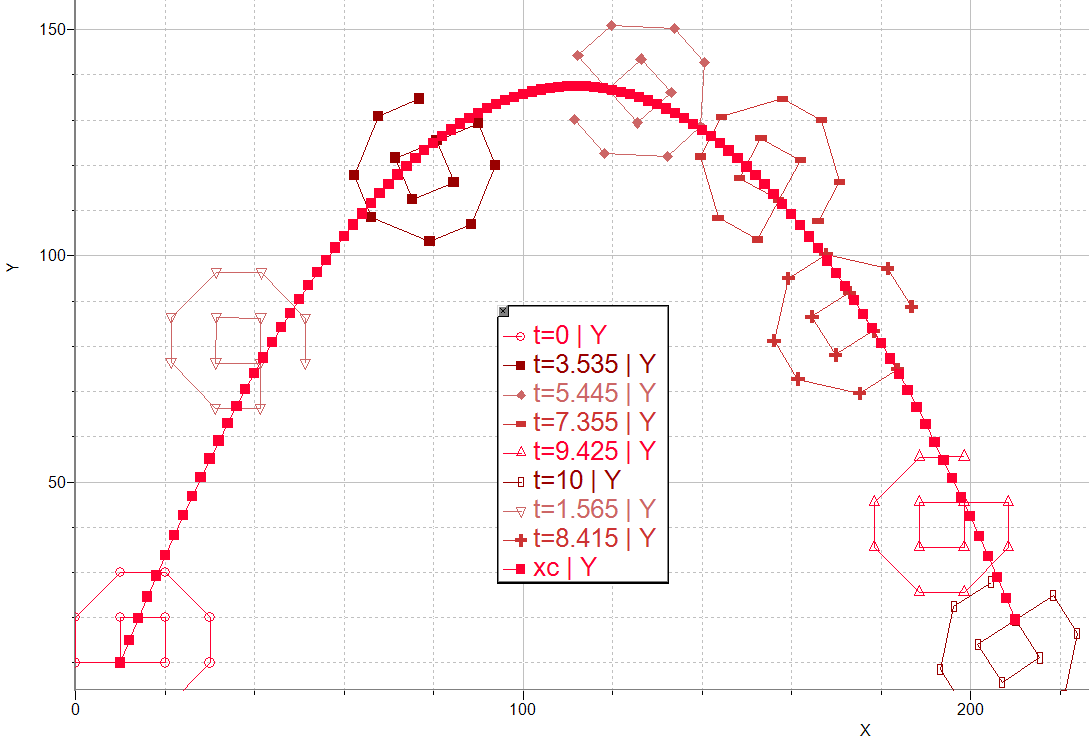
\includegraphics[width=\linewidth]{Pictures/xki_parabolic_12points.png}
  \caption{Пример расчета движения точек твердого тела}
  \label{fig:xki}
\end{figure}
\\Для более наглядной визуализации результатов расчет была реализована программа на языке программирования Python, которая создает анимацию движения твердого тела по предрассчитанным данным о положениях точек.
Результат работы данной программы прилагается в файле TestMovement.gif.

\subsection{Исследование сходимости}
Для расчета ошибки численного моделирования в данном примере было вычислено аналитическое решение.\\
Ошибка была рассчитана по норме $l_2$: как среднеквадратичное отклонение по следующей формуле:
\[
error_k=\sqrt{\sum_{i=0}^{stepN}||\overrightarrow{x}_k^i-\overrightarrow{x_{real}}_k^i||^2}
\]
Где $\overrightarrow{x_{real}}_k^i$ – положение k-ой точки твердого тела в момент времени $t=i\Delta t$, полученное из аналитического решения.\\
Ошибка расчета $\overrightarrow{x}_c$ - центра твердого тела:\\
Среднеквадратичное отклонение при вычислении 4000 шагов на отрезке времени 10с (длина временного шага 0.0025) составляет 2.47756e-10.\\
Ошибка расчета $\overrightarrow{x}_3$:\\
Среднеквадратичное отклонение при вычислении 4000 шагов на отрезке времени 10с (длина временного шага 0.0025) составляет 0.000469316.\\
Следует отметить сходимость рассчитанного решения к аналитическому: при измельчении шага $\Delta x$, значение ошибки $error_k$ стремится к 0:\\
\begin{figure}[h!]
  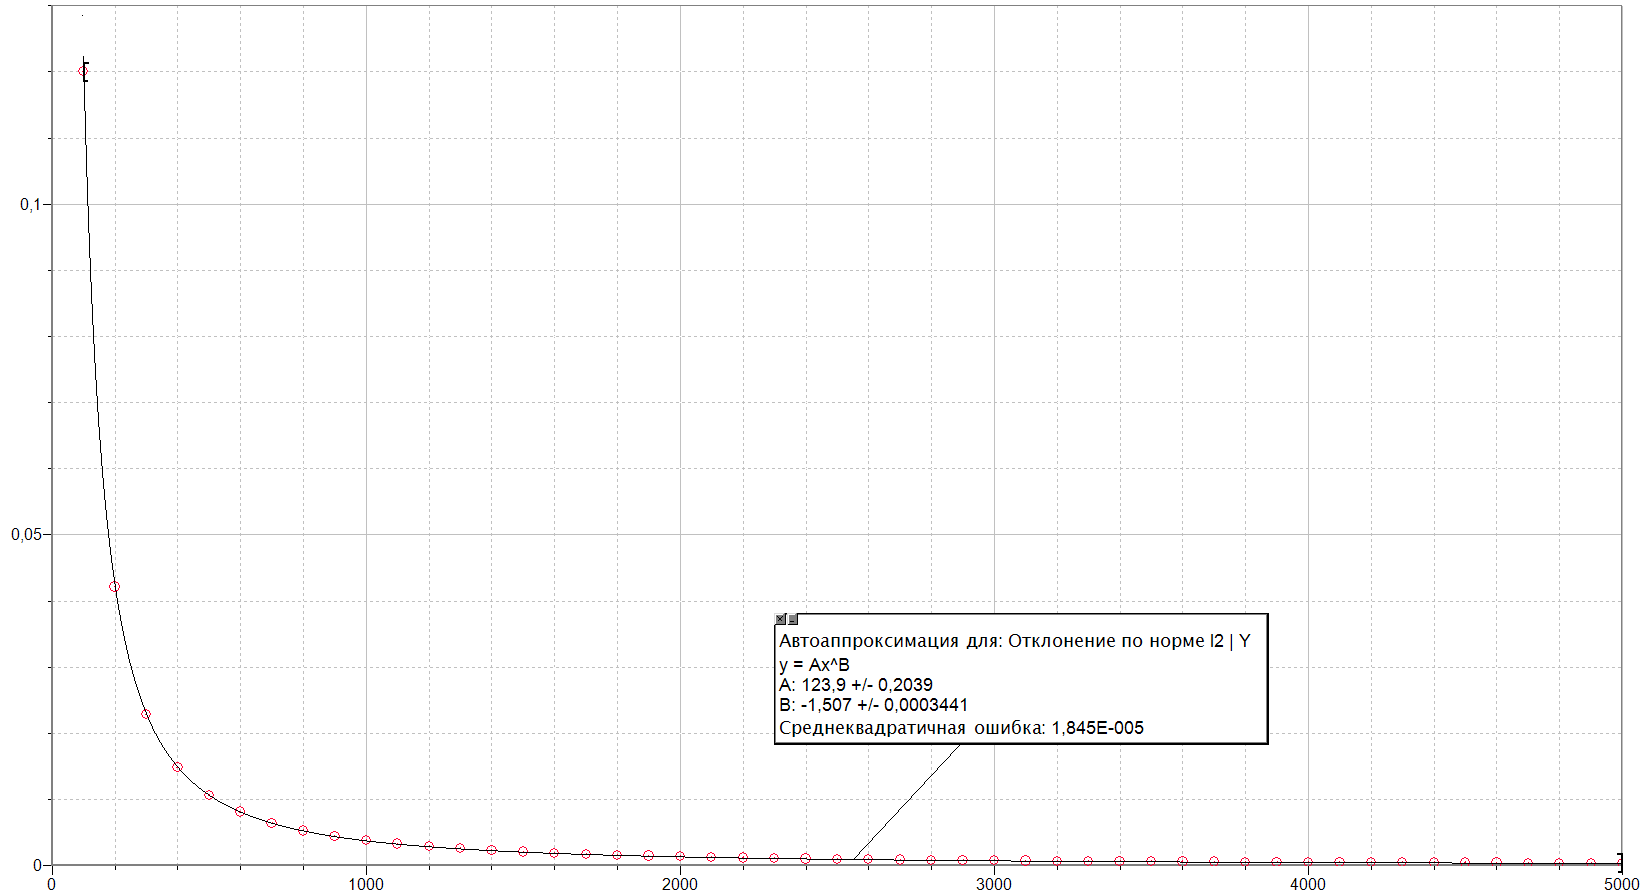
\includegraphics[width=\linewidth]{Pictures/dm_error_convergence.png}
  \caption{Сходимость метода DM. Среднеквадратичное отклонение при измельчении шага по времени}
  \label{fig:dm_err}
\end{figure}
.\\

\section{Численное решение уравнения переноса в одномерном случае со стационарным полем скоростей}
\subsection{Уравнение переноса}
\subsection{Теория}
\subsection{Численное решение}

\section{Численное решение уравнения переноса в одномерном случае с нестационарным полем скоростей}
\subsection{Уравнение переноса}
\subsection{Теория}
\subsection{Численное решение}

\section{Исследование различных схем}
\subsection{Метод Годунова(const)}
\subsection{Метод MUSCL (linear)}
\subsection{Метод THINC (tanh)}
\subsection{Метод JR (jump)}
\subsection{Исследование сходимости}

\section{Многомерное обобщение решения уравнения переноса с нестационарным полем скоростей}
\subsection{Расщепление по направлениям}
\subsection{Тестовые расчеты}

\section{Заключение}

\section{Список литературы}

\section{Приложения}
\subsection{Пример программного кода нахождения координаты центра твердого тела в моменты времени $t_i$}
\label{code:xc}
\begin{lstlisting}
function<Vector2D(vector<Vector2D>, double)> trapezoidQuadrature(){
    return [&](vector<Vector2D> f, double dx) -> Vector2D {
        return (f[0]+f[1])/2.*dx;
    };
}

void EESolver2DCenterStep(Vector2D& xc, const vector<Vector2D>& vc, int it,
const EESolver2DParams& params){
    if(it<=0) return;
    xc+=trapezoidQuadrature()({vc[it-1], vc[it]}, params.getDt());
}

void SolveEE2D(vector<Vector2D>& vertices, //vertices[0] is center
               const vector<Vector2D>& vc, const vector<double>& w,
               const EESolver2DParams& params, EESolver2DOutput& out){
    out.print(vertices, 0);
    for(int it=1; it<=params.getNTimeSteps(); it++){
        EESolver2DCenterStep(vertices[0], vc, it, params);
        //TODO solve for vertices here
        out.print(vertices, it);
    }
}
\end{lstlisting}

\subsection{Пример программного кода нахождения значений правой функции в моменты времени $t_i$}
\label{code:rf}
\begin{lstlisting}
Array<VectorXd, Dynamic, 1> integrateVector(Array<VectorXd, Dynamic, 1> f, double a, double b) {
    Array<VectorXd, Dynamic, 1> integral(f.size());
    double h = (b - a) / (f.size() - 1.);
    VectorXd i0 = VectorXd::Zero(f(0).size());
    integral(0) = i0;
    for (int i = 1; i < f.size(); i++) {
        integral(i) = integral(i - 1);
        integral(i) += (f(i - 1) + f(i)) * h / 2;
    }
    return integral;
}

function<VectorXd(double)> getRightFunc(function<VectorXd(double)> v, VectorXd xi0, function<Vector3d(double)> omega, function<VectorXd(double)> xc) {
    return [=](double t)->VectorXd {
        function<VectorXd(double)> integrand = [=](double tau)->VectorXd {
            VectorXd xcTau = xc(tau);
            Vector3d xcTau3(xcTau(0), xcTau(1), dimN < 3 ? 0 : xcTau(2));
            Vector3d crossProd = xcTau3.cross(omega(tau));
            VectorXd crossProdX(dimN);
            for (int i = 0; i < dimN; i++) crossProdX(i) = crossProd(i);
            return v(tau) - crossProdX;
        };
        return xi0 + integrateVector(integrand, 0, t, pow(10, -5), pow(10, -5));
    };
}

function<VectorXd(double)> getRightFuncNoMargin(function<VectorXd(double)> v, function<Vector3d(double)> omega, function<VectorXd(double)> xc) {
    return [=](double t)->VectorXd {
        function<VectorXd(double)> integrand = [=](double tau)->VectorXd {
            VectorXd xcTau = xc(tau);
            Vector3d xcTau3(xcTau(0), xcTau(1), dimN < 3 ? 0 : xcTau(2));
            Vector3d crossProd = xcTau3.cross(omega(tau));
            VectorXd crossProdX(dimN);
            for (int i = 0; i < dimN; i++) crossProdX(i) = crossProd(i);
            return v(tau) - crossProdX;
        };
        return integrateVector(integrand, 0, t, pow(10, -5), pow(10, -5));
    };
}
\end{lstlisting}

\subsection{Пример программного кода нахождения значений $x_k^i$}
\label{code:xk}
\begin{lstlisting}
Array<VectorXd, Dynamic, 1> getXi(function<VectorXd(double)> v,
VectorXd xi0,
function<Vector3d(double)> omega,
function<VectorXd(double)> xc, int stepsN, double h) {

    Array<VectorXd, Dynamic, 1> Xn(stepsN + 1);

    Array<VectorXd, Dynamic, 1> rightFuncCalc(stepsN + 1);
    function<VectorXd(double)> rightFunc = getRightFunc(v, xi0, omega, xc);
    for (int i = 0; i <= stepsN; i++)
        rightFuncCalc(i) = rightFunc(i * h);

    cout << "rightFuncCalc calculated" << endl;

    Xn(0) = rightFuncCalc(0);

    for (int k = 1; k <= stepsN; k++) {
        double sk = k * h;

        VectorXd innerSum(dimN);
        for (int i = 0; i < dimN; i++) innerSum(i) = 0;


        for (int j = 0; j < k; j++) {
            double sj = j * h;
            double Aj = (j == 0 ? 1. / 2. : 1.);

            VectorXd prodResult(dimN);
            Vector3d Xj(Xn(j)(0), Xn(j)(1), dimN < 3 ? 0 : Xn(j)(2));
            Vector3d crossProd = Xj.cross(omega(sj));
            for (int i = 0; i < dimN; i++) prodResult(i) = crossProd(i);

            innerSum += Aj * prodResult;
        }

        // Xk - h * innerSum(K-1) - h * Ak * [Xk ; OmegaK]  = rightFuncK
        // Xk - [Xk ; h * Ak *  OmegaK]  = rightFuncK + h * innerSum(K-1)
        // a - [a ; b] = c, a=?
        // ax - ay*bz = cx
        // ay + ax*bz = cy
        // (1 -bz)(ax)=(cx)
        // (bz  1)(ay)=(cy)
        // Ba=c, a = invB c

        Vector3d b = h * 0.5 * omega(sk);

        Vector2d rf2(rightFuncCalc(k)(0), rightFuncCalc(k)(1));
        Vector2d is2(innerSum(0), innerSum(1));
        Vector2d c = rf2 + h * is2;

        Matrix2d B; B <<
            1, -b(2),
            b(2), 1;

        Vector2d a = B.inverse() * c;

        VectorXd Xk(dimN);
        for (int i = 0; i < dimN; i++) Xk(i) = a(i);

        Xn(k) = Xk;
    }

    return Xn;

}
\end{lstlisting}

\subsection{Пример программного кода нахождения значений правой функции в моменты времени $t_i$}
\label{code:}
\begin{lstlisting}

\end{lstlisting}

\end{document}